%
% Use the standard article template.
%
\documentclass{article}

% The geometry package allows for easy page formatting.
\usepackage{geometry}
\usepackage{float}
\geometry{letterpaper}


% Load up special logo commands.
\usepackage{doc}

% Package for formatting URLs.
\usepackage{url}

% Packages and definitions for graphics files.
\usepackage{graphicx}
\usepackage{epstopdf}
\DeclareGraphicsRule{.tif}{png}{.png}{`convert #1 `dirname #1`/`basename #1 .tif`.png}

%
% Set the title, author, and date.
%
\title{Headmaster Dream Design}
\author{Eric Dea}
\date{November 29, 2012}


%
% The document proper.
%
\begin{document}

% Add the title section.
\maketitle

% Add an abstract.
\abstract{
This paper explains how skeuomorphic interface designs fit the user's and developer's mental model.  Skeuomorphic designs are intended to create a familiar layout for users, especially new or novice users.  Effectively aligning user and developer mental models is exactly what skeuomorphism is about. When trying to create an effective usable interface, skeuomorphism comes to the mind of the developer.  This paper will show that the usability of skeuomorphic user interface designs is directly related to the successful alignment of the user and developer mental models.}

% Add various lists on new pages.
\pagebreak
\tableofcontents

\pagebreak
\listoffigures

\pagebreak

%
% Body text.
%
\section{Introduction}
\label{introduction}

A Skeuomorph, or Skeuomorphism, is when a product imitates design elements functionally necessary in the original product design, but that becomes ornamental in the new product design \cite{wiki}.  So in the computer world, a skeuomorphic user interface design is one that tries to imitate a 'real world' interface by using various decorations.  The website interface designer tries to replicate what the user's mental model is, what the user pictures in their mind.  This relationship between the user's mental model and the developer's mental model is key to creating most successful user interfaces.  Some interfaces, especially ones that rely on usability, want the skeuomorphic interface design to also function like the real world counterpart, not just imitating the looks.  In this paper, I hope to show how important this relationship is and how skeuomorphism directly relates to this relationship between the user and developer's mental models.


\section{Skeuomorphism}

In a User Interface, the elements of the interface can either be functional or non-functional.  The functional elements can either be skeuomorphs or just plain old elements that are necessary to the interface.  The non-functional elements are there for decoration and visual satisfaction.  This is where skeuomorphs come into play, for they create a better looking layout for most novice computer users.

\subsection{Non-Functional Elements}

Skeuomorphism, or skeuomorphs, have a certain abstract quality and property.  The layout and content of a user interface must have components that can be made abstract, or nonfunctional.  An abstract component can serve both as a building block for new development and as a reminder of its future functionality \cite{skeu-software}. So, even though most of these 'abstract' elements are non-functional and are just decorations, there is an option for future development to make these elements functional.  An example of this abstract element, or non-functional, is the rip/tear on Apple's iCal.

\begin{figure}[H]
\centering
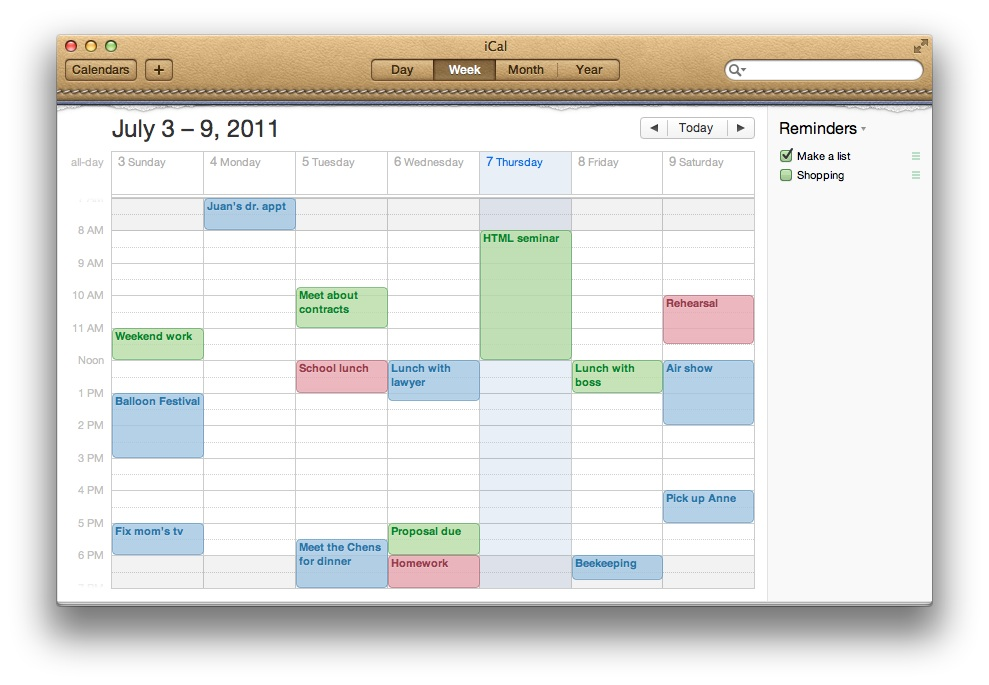
\includegraphics[width=3.5in]{ical.jpeg} 

\caption{iCal with Skeuomorphism}
\label{iCal}
\end{figure}

If you look at the top of Figure \ref{iCal}, there are rip marks indicating that the user 'ripped' out the past month, just like an ordinary calendar.  The tear has no functionality, for it is just there for decoration.

\subsection{Functional Elements}

On the other side of Skeuomorphism, there are elements of a user interface that exactly replicate the real life version and also have functionality.  One common example of this is Figure \ref{traktor}, which is a DJ mixing software Traktor.

\begin{figure}[H]
\centering
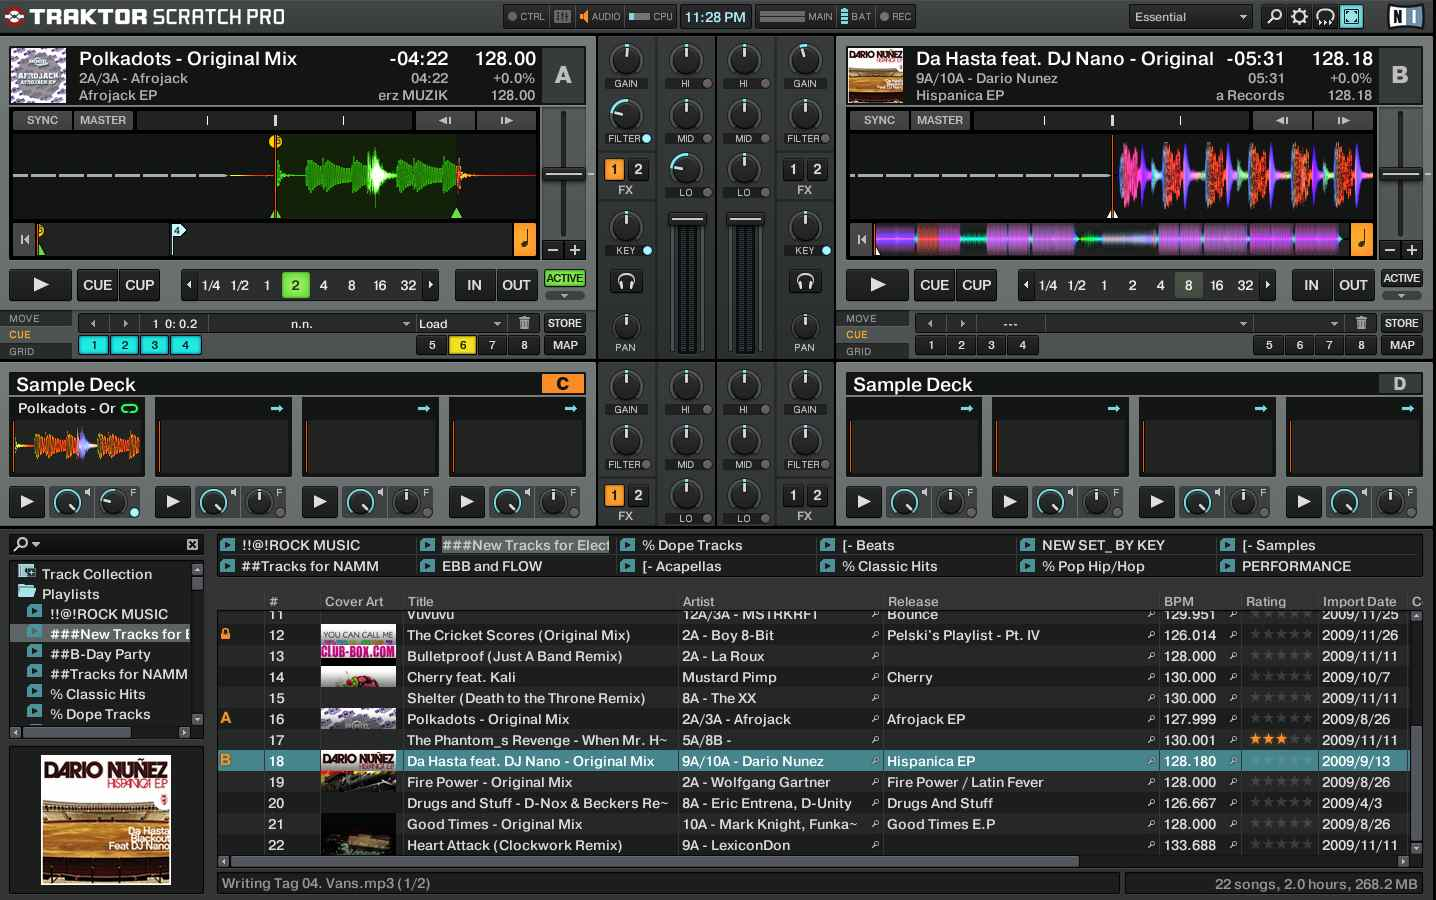
\includegraphics[width=4.5in]{traktorUI.jpg} 

\caption{Traktor Scratch Pro 2}
\label{traktor}
\end{figure}

All of the buttons and knobs on the interface are fully functional.  A DJ mixing set has very similar, if not exact, buttons and knobs.  Because all of the knobs are turned just like a real DJ mixer, the skeuomorphic elements are functional.  A skeuomorphic user interface where all of its elements are functional is the perfect interface where the user's mental model and the developer's mental model is on the same page.  For example, say the user is a DJ who uses mixers but has not ever DJed on a computer.  If this user were to try out this digital interface, the transition is very easy for everything on his own mixer looks and works exactly the same on the computer.

\section{Mental Model}

A mental model is an explanation of someone's thought process about how something works in the real world \cite{wiki-mental}.  When trying to successfully align the mental models of the user and the developer, their thought processes must be similar.  Because skeuomorphism is the imitating of elements to a new product, the quality of the skeuomorphism is directly related to the developer's alignment of the mental model of the user.  If done well, skeuomorphism can improve the user interface by providing a familiar mental model to the user.

\subsection{Apple's View on the Mental Model}
The user already has a mental model of any given software.  This mental model comes from real world experiences, experience with the software/interface and the experience with computers in general \cite{apple}.  When trying to create an interface, Apple suggests the follow characteristics:

\begin{itemize}
\item Familiarity
\item Simplicity
\item Availability
\item Discoverability 
\end{itemize}

These four characteristics are great guidelines for trying to fit the user's mental model.  Almost all of Apple's products reflect these characteristics, and whether they are good or not is determined by the user.  There are both positive and negative examples of using skeuomorphic interfaces when trying to capture the user's mental model.

\subsubsection{Positive Examples}

In Figure \ref{apple-metro}, Apple's Notes app and Microsoft's Notes app are being compared.  Apple provides a clean familiar feel to both new and experienced users, while Microsoft's Metro looks very simplistic and modern.  The Metro, to some people, can feel impersonal for they are not familiar with how to take notes on a phone.  Any new user to a smartphone would pick up and recognize Apple's Notes app way faster than the Metro.  The app is also very usable because the user knows instantly that this is a notepad and one can essentially "take notes" on it.  This is all because of Apple's skeuomorphic interface design in alignment with the user's mental model.

\begin{figure}[H]
\centering
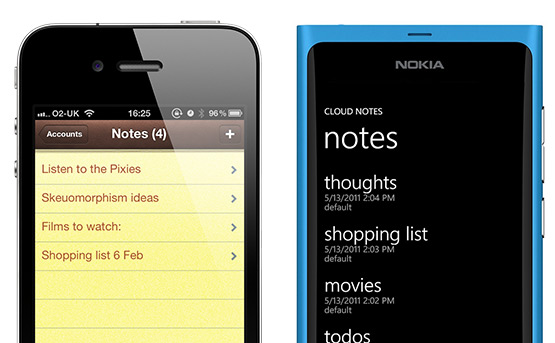
\includegraphics[width=4.5in]{iphone-metro.jpg} 

\caption{Apple's iPhone vs Microsoft's Metro}
\label{apple-metro}
\end{figure}

\subsubsection{Negative Examples}

Apple is a company that uses skeuomorphic designs a lot in their products. Such examples are the iCal, Notes (iPhone), folder icons to indicate folders, and iBooks/Newsstand.  While this might fit the mental model of people who are new to the world of computers, there are a lot of complaints by experienced users who feel that the skeuomorphic interface does not fit their mental model. 

One example is about iCal's design: "iCal�s leather-stitching was literally based on a texture in [Steve Jobs'] Gulfstream jet," SVP of Industrial Design Jony Ive said. "There was lots of internal email among UI designers at Apple saying this was just embarrassing, just terrible \cite{apple-insider}."  Even though a skeuomorphic design may look cleaner and nicer, the functionality and utility could be bad.  In comparison to Apple's calendar on the iPhone, the calendar app on the iPhone (Figure \ref{iphone-cal}) uses a simplistic, efficient design that is not as skeuomorphic as the iCal.

\begin{figure}[H]
\centering
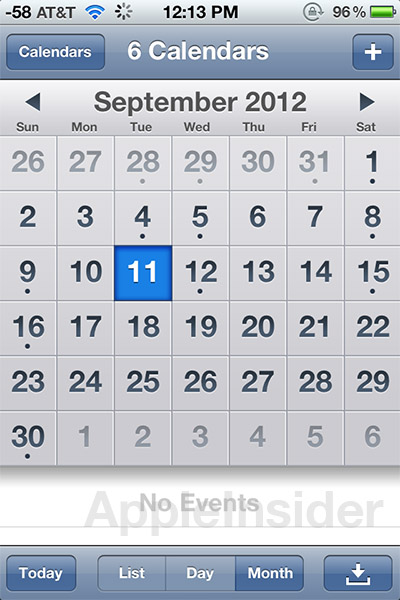
\includegraphics[width=2in]{iphone-cal.jpg} 

\caption{Apple's iPhone Calendar}
\label{iphone-cal}
\end{figure}

The usefulness of a user interface is very important to almost all users, especially frequent users.  One of Apple's designers, Yves B�har, shares his thoughts about the Bookshelf and Newsstand apps: \begin{quote}I�ve come to absolutely dislike this trend in user interface toward skeuomorphism. Using reality as a visual metaphor for the user interface rather than make the UI function on its own terms is something that has irked me for quite a while.  The digital bookshelf doesn�t really work like a bookshelf, Behar said. You�re throwing all this extraneous visual noise at me and it�s confusing. My brain, which is used to the physical bookshelf, is confused because of the differences in usability. It�s cute, but not particularly useful. \cite{apple-insider}\end{quote}

Even though the interfaces of the Bookshelf and Newsstand apps fits the mental model of the user well, their own designers are complaining about how skeuomorphic interfaces are not always the best way to fit the mental model.  This quote is an example where the user, Yves Behar, notices the skeuomorphic design is more visually based rather than usability based.  If the apps worked and acted more like their real world counterparts, they would fit Behar's mental model more closely.

\section{Conclusion}

Skeuomorphic designs are meant to fit the mental model of the user.  This means that the looks and functionality must be similar to what the user's thought process is.  Creating a successful user interface in line with the user's mental model is what skeuomorphism is all about.  Skeuomorphisms are elements of the new product that try to imitate the elements of the original product.  By imitating these elements, the user instantly feels familiar with the software.  In addition to just looks, the skeuomorphic interface must also have the same functionality in order to successfully align with the mental model of the user.  The first thing a new user sees is the design, then the user tries to use it.  So, in order for the interface to be successful, it must also be usable.  If the skeuomorphic user interface design is familiar and usable, then the mental model of the developer and the user are perfectly aligned.

% Generate the bibliography.
\bibliography{cmsi370-skeuomorphic}
\bibliographystyle{unsrt}

\end{document}
